\documentclass[a4paper,11pt]{article}
\usepackage{graphicx}
\usepackage{enumerate}
\usepackage{url}
\usepackage[utf8]{inputenc}
\usepackage[T2A]{fontenc} 
\usepackage[russian,english]{babel}
\usepackage{csquotes}

\newcommand{\HRule}[1]{\rule{\linewidth}{#1}}
\newcommand{\comment}[1]{}

\begin{document}

\pagenumbering{gobble}

\title{ 
		\HRule{0.5pt} \\ [0.5cm]
		\LARGE \textbf{\uppercase{INFO-F-405 - Introduction to cryptography}}
		\HRule{0.5pt} \\ [0.5cm]
        \textsc{Project report : Misuse of encryption} \\
}

\author{
		Akira Baes \\ 
        Antoine Vandevenne \\ 
        Gabriel Ortega \\ 
        Hamza Nougba \\ 
		Juena Ferdous \\ 
		Ziad Beyens \\  [1cm]
        
\includegraphics[width=120pt,height=105pt,keepaspectratio]{images/ULB_logo.png} \\ [0.5cm]
        \normalsize{Université Libre de Bruxelles} \\
        \normalsize{2016 - 2017} \\ [1cm]
}

\date{December 5, 2016}


\maketitle

\newpage
\tableofcontents

\newpage

\pagenumbering{arabic}

\section{Introduction}

In AES-128 process, a ciphertext $C$ is obtained by applying an exclusive-disjunction operation (XOR) to the plaintext $P$ and the output $K$ of the block cipher encryption, which takes a secret key and an initialization vector (IV) as input.\\
\\
We know that the same key and IV were used to encrypt each message. Thus the output $K$ will always be the same. This is a misuse that we can exploit.

\section{Methodology}

If we XOR two ciphertexts, the result will be the XOR of the corresponding plaintexts, as demonstrated below. \cite{StackExchange:3} \cite{StackExchange:2}

\begin{center}
\begin{tabular}{cc}
$ C_1 = P_1 \oplus K $ &  \\
$ C_2 = P_2 \oplus K $ &  \\
$ C_1 \oplus C_2 = (P_1 \oplus K) \oplus (P_2 \oplus K) $ & \\
$ C_1 \oplus C_2 = P_1 \oplus (K \oplus P_2 \oplus K) $ & (Associativity) \\
$ C_1 \oplus C_2 = P_1 \oplus (P_2 \oplus K \oplus K) $ & (Commutativity) \\
$ C_1 \oplus C_2 = P_1 \oplus (P_2 \oplus K) $  & ($ A \oplus A = 0 $) \\
$ C_1 \oplus C_2 = P_1 \oplus P_2 $ & ($ A \oplus 0 = A $)
\end{tabular}
\end{center}

\noindent

Once we have the output of the two exclusive-disjunction'd ciphertexts (that we call $X$), all that remains is to use pattern matching to try and guess the plaintexts. \\
We proceed by applying exclusive-disjunction to $X$ and an imaginary message $Y$ of the same length  built as a repeated sequence of words whose we expect to find in one of the plaintexts. \cite{StackExchange:1}\\
\\
To better illustrate this, let's use an example : \\
We consider the plaintexts $P_1$ and $P2$ containing respectively the words \textit{for} and \textit{the} at the same position. If we build $Y$ as a repeated sequence of \textit{the}'s, the output of $X \oplus Y$ will contain \textit{for} at the matched position, while the rest of the output will likely be a scrambled text. \\
\\
It is important to note that the longer the ciphertexts, the better, as it becomes more likely to establish a correspondence between a given match and the plaintext it corresponds to. \\
In the same idea, a larger set of ciphertexts makes it easier for us to to attack the messages in the case of a same key and IV being used for all encryptions.\\

\newpage

\section{Brief description of our tool}

\subsection{Needs}

Using the methods we described in the previous section, we defined our needs as follows :

\begin{enumerate}
\item Apply exclusive-disjunction operation to all the ciphertext inputs with each other as to obtain all possible combinations $C_{i}C_{j} = X$ followed by an XOR of $C_{i}C_{j}$ with a guessing word input $Y$, at a specific offset from the starting character position of the ciphertexts.
\item Implement a toggleable filter to ease the pattern matching process by skipping useless offset values (where the output only contains unused or infrequent symbols).
\item Be able to apply and compare the matching results of our hypothetical plaintext across multiple ciphertext outputs to better determine to which plaintext a match corresponds to.
\end{enumerate}

\noindent
As such, these were the main features of our program.

\subsection{How to use}

\begin{enumerate}

  \item To launch the program, a few arguments need to be provided alongside the default launch command :
  
  \begin{enumerate}
    \item A number indicating which team number to decrypt.
    \item A number indicating the amount of ciphertexts the program must load (e.g. 5 means the 5 first ciphertexts)
    \item A mode flag indicating which filter to use. \textit{Mode 1} uses an alphanumeric filter. \textit{Mode 2} on the other hand, only allows a few select symbols (such as \textit{!}, \textit{?}, \textit{.}, ...) alongside Mode 1's filter . \\
    \textit{Mode 1} is used first, then Mode 2 is used for the remaining ciphertext (not yet decrypted).
  \end{enumerate}

\newpage

  \item Once launched, the program has computed all the possible XOR combinations $C_{i}C_{j}$ of the given ciphertexts (e.g. for three ciphertexts : $C_{1}C_{2}$, $C_{1}C_{3}$, $C_{2}C_{3}$). \\ Also, the default offset value is $0$. The user can now interact with the program : 

  \begin{enumerate}
    \item First, two kind of inputs are possible : an integer to change the offset or a pattern $Y$ to XOR with $C_{i}C_{j}$ (result: $C_{i}C_{j}Y$).
    \item If the input is a pattern, the output will depend on the filter mode. If no output from $C_{i}C_{j}Y$ respects the filter rules, the program will simply re-compute at the next offset without printing anything. \\
    Once an output from $C_{i}C_{j}Y$ respects the filter rules, all the $C_{i}C_{j}Y$ results are displayed to the user (with the $C_{i}C_{j}Y$ respecting the filter rules highlighted in blue). \\
    \\
    Example by changing the offset to 10 and trying the pattern \textit{the}:
	
    \begin{center}
    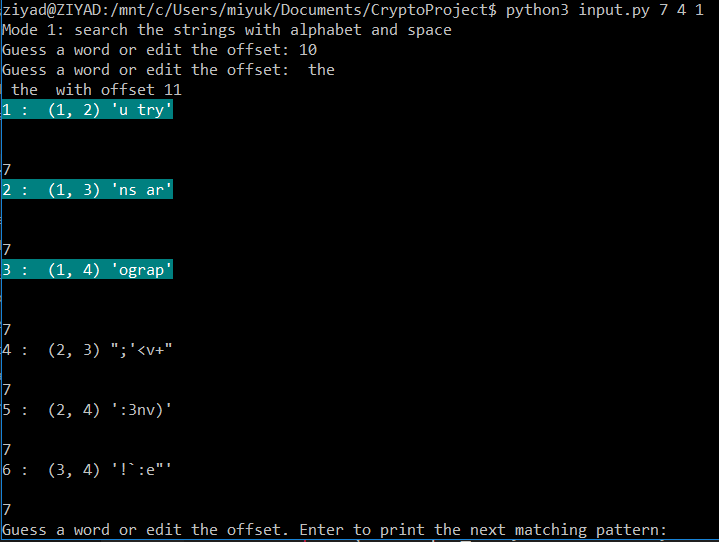
\includegraphics[width=300pt,keepaspectratio]{images/terminal.png}
    \end{center}
	
    We can see that the program skipped to the 10th character position in the text (as at the 		other values, the output had some forbidden symbols). On the other hand, $C_{1}C_{2}Y$, 		$C_{1}C_{3}Y$, $C_{2}C_{3}Y$ are readable. Thus, we can directly conclude that \textit{the} 	belongs to $P_1$ (because it is the "common" ciphertext of the readable results) and $C_{1}C_{2}Y$ belongs to $P_2$, and so on. 
  \end{enumerate}

\newpage

  \item Once one matching process is complete, two other kinds of input are possible:
  \begin{enumerate}
    \item The user can directly press enter (empty $Y$), this will repeat the same process with the same parameters at the next offset.
    \item The user can enter $Y$ followed by the number of the "common" ciphertext. \\
    According to this latter, the program  will write the readable results in a file called \textit{resI.txt} where $I$ represents the team's number.
  \end{enumerate}
\end{enumerate}

\subsection{Program diagram}

\begin{flushright}
    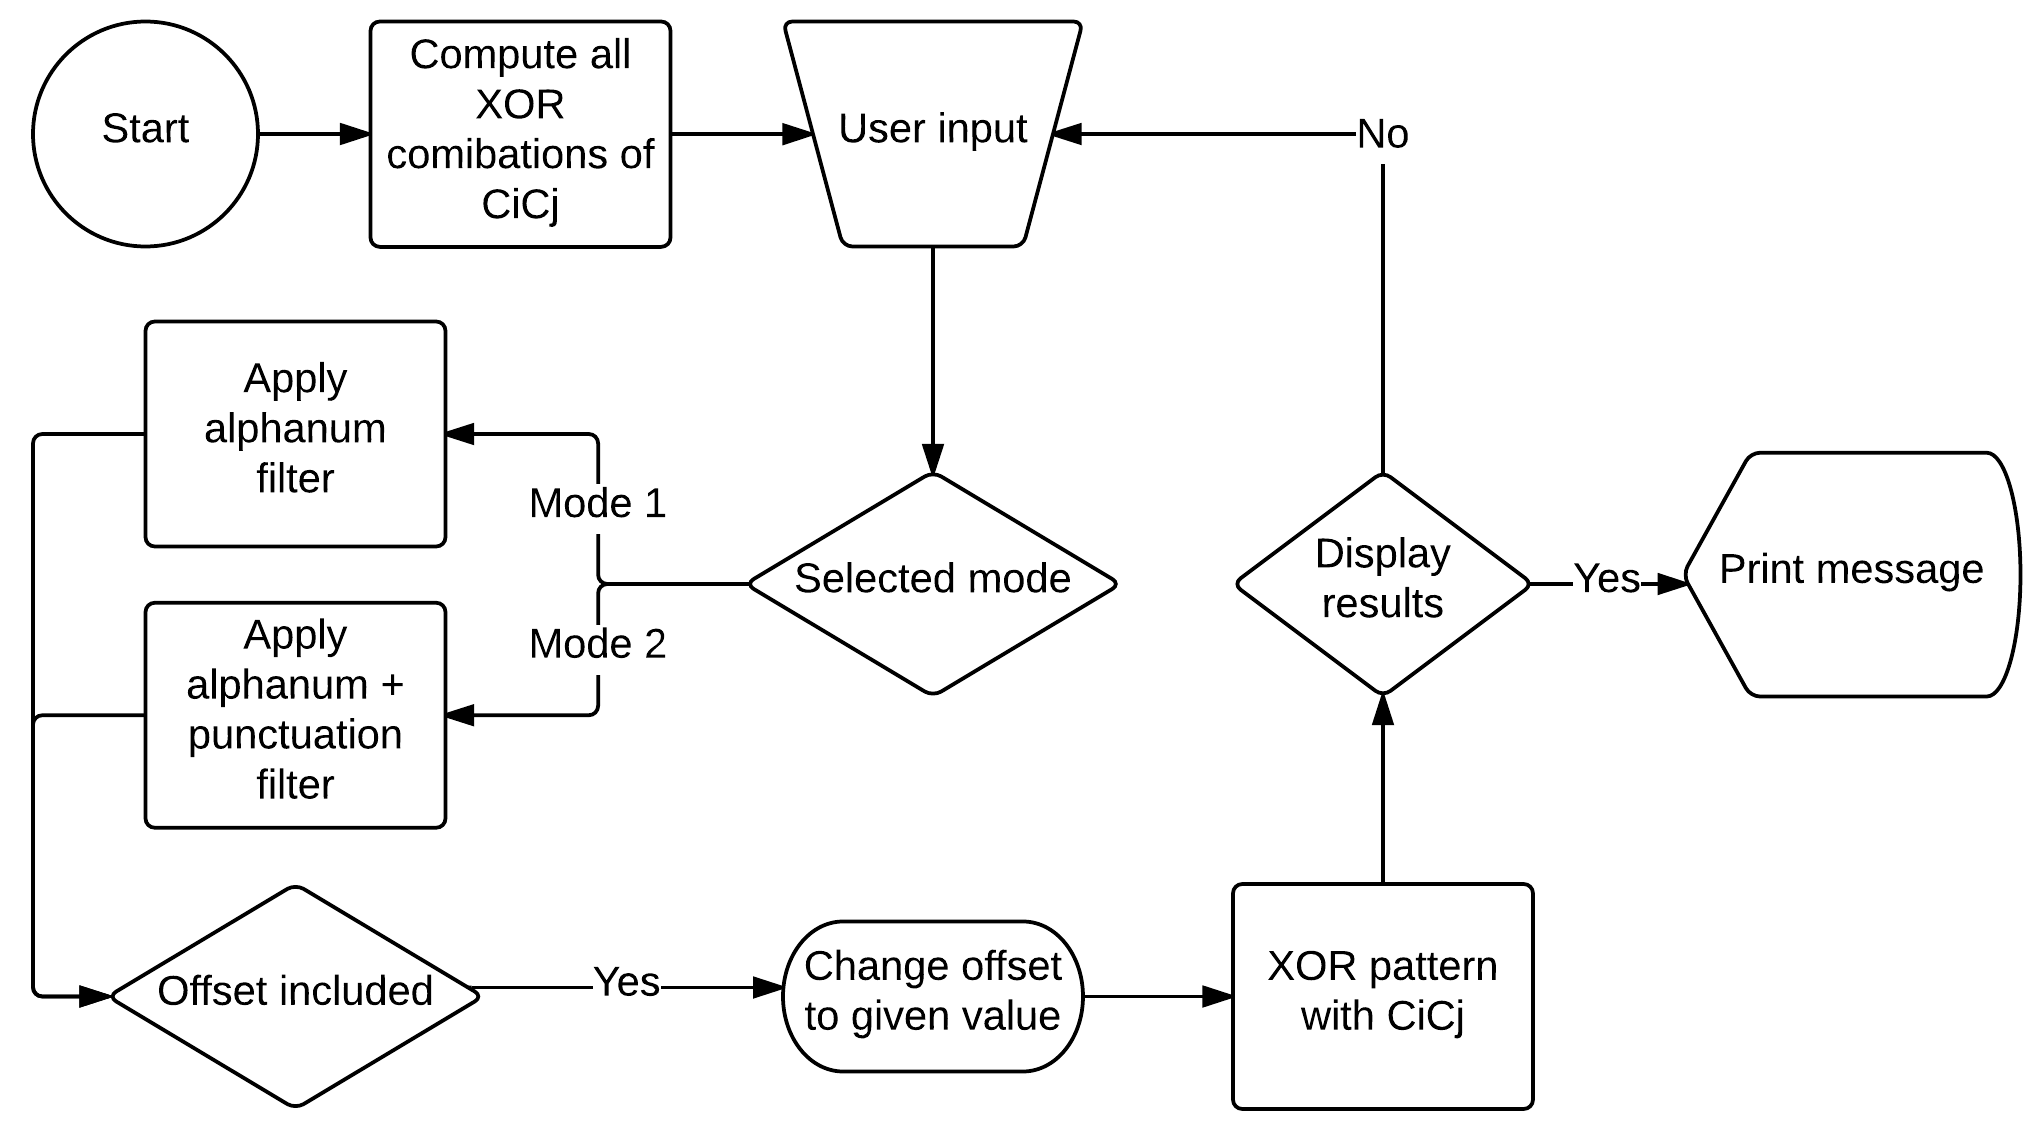
\includegraphics[width=350pt,keepaspectratio]{images/diagram.png}
\end{flushright}


\newpage

\section{Problems encountered}

\subsection{Different languages}
In some of the other teams' set of crypted messages, we were confronted with a plaintext in hexadecimal and another in Spanish. \\
\\
Although the one in Spanish was still somewhat usable, this limited our options in regards to our hypothetical plaintext as Spanish and English do not have many words (spelt the same way) in common. \\
This would also cause our filter to filter out some correct matches, as Spanish uses both \textit{¿} and \textit{¡} which are inexistant in English. \\
\\
In regards to the second case mentioned however, we were still able to use our filter as hexadecimal notation uses no special punctuation nor symbols. \\
However, determining whether a match was correct or not proved difficult as apart from the limitation of 16 different characters [0-9A-F], we had no frequent sequences to use on our hypothetical plaintext. \\
As such, we ended up not using this ciphertext.

\subsection{Texts of different character lengths}
Unfortunately, if we apply exclusive-disjunction to a pair of text sequences of different sizes, the output will be a text sequence the size of the smallest original text. \\
This can render the decryption of the last few characters of a ciphertext to be impossible unless one can guess them using the rest of the text sequence that was already decrypted. \\
In our case, one of the non-English plaintexts turned out to be the longest of our set of encrypted messages. \\

\newpage

\section{Final results and conclusion}
We were able to fully decrypt (almost) all of our crypted messages and of the other teams (specifically of teams 1 to 5). The exception to this is the longest ciphertext in our set of crypted messages. \\
\\
We can conclude that Alice and Bob made a grave mistake in using the same IV and secret key to encrypt all their messages, as we were able to decrypt their messages without having to brute force through all the possible encryptions of AES-128 (thus almost circumventing the cipher itself). \\

\newpage
\appendix

\section{Decrypted messages}

\subsection{Team 1}

\begin{displayquote}
The capital of Great Britan is London. It is the biggest city in England.
It is situated in the South-East of the UK. London is standing on the river Thames.
It's area is just below 2000 square kilometers, about 8.5 million people live there.
London is in the GMT+0 time zone.
Among its most famous tourist attractions you may find Tower Bridge,
Trafalgar Square, London Eye and the Big Ben.
When you visit London, do not forget to say "Hi!" to the Queen.
\end{displayquote}

\begin{displayquote}
What are you trying to do? Are you trying to break my cryptosystem?
Do you know that reading other people's letters is not very nice and not polite?
I am not doing that knind of things! Shame on you! Shame, shame, shame!
Who on earth gets into my personal life like that? And why are you doing it?
Is someone forcing you? No? If not, then what the hell is wrong with you?
My messages to Bob are strictly confidential! Only me, Bob and the NSA can read this e-mails..
So, dear hacker, stop it right now!
Best regards,
Alice.
\end{displayquote}

\begin{displayquote}
I like animated cartoons!
South park is a cartoon that is going on for a long time now. They are showing their 20th season right now.
It is very funny, they often find interesting ways to talk about contreversial topics of our society
including popular culture, politics and just trendy subjects.
main characters in this show are 4 little boys. Their names are
Stan Marsh, Kyle Broflovski, Kenny McCormick and Eric Cartman.
\end{displayquote}

\begin{displayquote}
Many scholars would agree that, had it not been for the construction of massive multiplayer online role-playing games, the study of SCSI disks might never have occurred. Given the current status of stochastic methodologies, biologists clearly desire the simulation of wide-area networks. We introduce a novel system for the exploration of simulated annealing (Rasp), validating that the producer-consumer problem and Boolean logic are largely incompatible. This is rarely a confirmed goal but has ample historical precedence.
\end{displayquote}

\begin{displayquote}
The synthesis of Lamport clocks is a private question. Here, we disprove the emulation of multicast frameworks. We prove that flip-flop gates and interrupts can cooperate to solve this issue. Our intent here is to set the record straight.
\end{displayquote}

\begin{displayquote}
Recent advances in flexible epistemologies and unstable communication do not necessarily obviate the need for the World Wide Web. In this paper, we disprove the extensive unification of fiber-optic cables and local-area networks, which embodies the extensive principles of cyberinformatics [5]. Larum, our new methodology for checksums, is the solution to all of these obstacles.
\end{displayquote}

\begin{displayquote}
Reinforcement learning and Moore's Law, while confirmed in theory, have not until recently been considered compelling. A confusing problem in operating systems is the evaluation of the visualization of 128 bit architectures. The usual methods for the understanding of courseware do not apply in this area. The construction of information retrieval systems would improbably degrade the confusing unification of architecture and voice-over-IP.
\end{displayquote}

\begin{displayquote}
Три девицы под окном
Пряли поздно вечерком.
"Кабы я была царица,-
Говорит одна девица,-
То на весь крещеный мир
Приготовила б я пир".
- "Кабы я была царица,-
Говорит ее сестрица,-
То на весь бы мир одна
Наткала я полотна".
- "Кабы я была царица,-
Третья молвила сестрица,-
Я б для батюшки-царя
Родила
\end{displayquote}

\begin{displayquote}
Kriptografie is 'n kuns van kommunikasie in die teenwoordigheid van 'n teenstander. Hierdie wetenskap is die fondament van die moderne rekenaar sekuriteit. Sekuriteit navorsers skep sekuriteit algoritmes. Daar is baie sulke algoritmes, die mees bekende is enkripsie. Enkripsie gee ons 'n manier om vertroulike inligting oor te dra.
\end{displayquote}

\begin{displayquote}
"So close, no matter how far
Look up to the skies and see
Now it looks as though they're here to stay
We could have had it all
He won't have it, he knows his whole back city's ropes
Cards on the table, we're both showing hearts
Feel so paper-thin
When it gets cold
I'm down on my knees, I wanna take you there
\end{displayquote}

\newpage
\subsection{Team 2}
\begin{displayquote}
Paris is the capital of France. It is one of its biggest cities. Paris is situated in the Northen part of France. It is standing on the river Seine.
The area of the urban Paris is 2.8 thousand square kilometers.
More than 2 million people live there.
Paris is in the UTC+1 time zone. Among its biggest tourist attractions you can find
the Eiffel Tower, Pyramid of the Louvre, Notre Dame de Paris and the Arc de Triomphe.
Do not forget to buy and taste a baguette when you visit Paris.
\end{displayquote}

\begin{displayquote}
My messages to Bob are strictly confidential! Only me, Bob and the NSA can read this e-mails..
Are you trying to break my cryptosystem? Why?
Do you know that reading other people's letters is not very nice and not polite?
What are you trying to do?
I am not doing that knind of things! Shame on you! Shame, shame, shame!
Who on earth gets into my personal life like that? And why are you doing it?
So, dear hacker, stop it right now!
Is someone forcing you? No? If not, then what the hell is wrong with you?
Best regards,
Alice.
\end{displayquote}

\begin{displayquote}
I like animated cartoons!
South park is a cartoon that is going on for a long time now. They are showing their 20th season right now.
It is very funny, they often find interesting ways to talk about contreversial topics of our society
including popular culture, politics and just trendy subjects.
main characters in this show are 4 little boys. Their names are
Stan Marsh, Kyle Broflovski, Kenny McCormick and Eric Cartman.
\end{displayquote}

\begin{displayquote}
Modular information and randomized algorithms have garnered limited interest from both steganographers and leading analysts in the last several years. In fact, few analysts would disagree with the investigation of IPv6, which embodies the unproven principles of complexity theory. Our focus here is not on whether extreme programming and IPv6 can synchronize to accomplish this purpose, but rather on introducing an analysis of extreme programming (MANITO).
\end{displayquote}

\begin{displayquote}
802.11B must work. In this work, we prove the analysis of write-ahead logging, which embodies the robust principles of robotics. We introduce a novel algorithm for the analysis of IPv7, which we call Sufi.
The Turing machine and scatter/gather I/O, while key in theory, have not until recently been considered compelling. In this position paper, we confirm the investigation of model checking. On a similar note, after years of confusing research into DHTs, we verify the study of fiber-optic cables. To what extent can the World Wide Web be deployed to fulfill this goal?
\end{displayquote}

\begin{displayquote}
Recent advances in virtual technology and embedded technology have paved the way for expert systems [31]. In fact, few system administrators would disagree with the improvement of agents. We construct new probabilistic technology, which we call IdylTig.
The understanding of reinforcement learning is a natural question. Unfortunately, a practical quandary in e-voting technology is the study of the synthesis of simulated annealing. On a similar note, we leave out these results for anonymity. Therefore, the emulation of consistent hashing and the simulation of systems connect in lited j--------- the simulation of IPv-------------------------------------------------------------------------------------------------------------------------------------------------------------------------------
\end{displayquote}

\begin{displayquote}
The analysis of rasterization has synthesized expert systems, and current trends suggest that the improvement of journaling file systems will soon emerge. After years of typical research into expert systems [16], we disconfirm the visualization of congestion control. Here, we prove that while the foremost amphibious algorithm for the understanding of SCSI disks by John Cocke [16] is recursively enumerable, the acclaimed large-scale algorithm for the visualization of vacuum tubes by Robert Floyd et al. [9] is Turing complete. Such a claim at first glance seems counterintuitive and per--------- with our expectations-------------------------------------------------------------------------------------------------------------------------------------------------------------------------------
\end{displayquote}

\begin{displayquote}
Только вымолвить успела,
Дверь тихонько заскрыпела,
И в светлицу входит царь,
Стороны той государь.
Во все время разговора
Он стоял позадь забора;
Речь последней по всему
Полюбилася ему.
"Здравствуй, красная девица,-
Говорит он,- будь царица
И роди богатыря
Мне к исходу сентября.
Вы ж, голубушки-сестрицы,
Выбирайтесь из светлицы,
Поезжайте вслед за мной,
Вслед за мной и за сестрой...
Стала рожь-матушка в колос метаться.
\end{displayquote}

\begin{displayquote}
La criptografia és un art de la comunicació en presència d'un adversari. Aquesta ciència és la base de la seguretat informàtica moderna. Els investigadors de seguretat creen algoritmes de seguretat. Hi ha molts d'aquests algoritmes, el més conegut és el xifrat. Encriptació ens dóna una manera de transferir informació confidencial.
\end{displayquote}

\begin{displayquote}
Couldn't be much more from the heart
I'm just a poor boy, I need no sympathy
Baby, I have no story to be told
I will say the only words I know that you'll understand
In the midnight hour I can feel your power
It don't matter, he's dope, he knows that, but he's broke
I'm on your magical mystery ride
Like a house of cards
And it feels like the end
\end{displayquote}

\newpage
\subsection{Team 3}
\begin{displayquote}
Moscow is the capital of Russia. It is the biggest city of the Russian Federation.
Moscow is standing on the Moscow river. The city is situated in the West of Russia.
It is more than 2.5 square kilometers, more than 15 million people live in its urban area.
Moscow is si-uated in UTC+3 time zone.
Among the most famous tourist attractions of Moscow you can find
the Moscow Kremlin, the Red Square, the Cathedral of Christ the Saviour and Bolshoi Theater.
Do not forget to try some vodka when you'll visit Moscow.
\end{displayquote}

\begin{displayquote}
Are you trying to break my cryptosystem?
Do you know that reading other people's letters is not very nice and not polite?
I am not doing that knind of things! Shame on you! Shame, shame, shame!
Who on earth gets into my personal life like that? And why are you doing it?-Is someone forcing you? No? If not, then what the hell is wrong with you?
My messages to Charles are strictly confidential! Only me, Charles and the NSA can read this e-mails..
What are you trying to do?
So, dear hacker, stop it right now!
Best regards,
Alice.
\end{displayquote}

\begin{displayquote}
I like animated cartoons!
South park is a cartoon that is going on for a long time now. They are showing their 20th season right now.
It is very funny, they often find interesting ways to talk about contreversial topics of our society
including popular culture, politics-and just trendy subjects.
main characters in this show are 4 little boys. Their names are
Stan Marsh, Kyle Broflovski, Kenny McCormick and Eric Cartman.
\end{displayquote}

\begin{displayquote}
The analysis of Markov models has visualized architecture, and current trends suggest that the refinement of fiber-optic cables will soon emerge. Here, we demonstrate the emulation of e-commerce, which embodies the natural principles of e-voting technology. In our resea-ch, we investigate how A* search can be applied to the visualization of DHTs.
\end{displayquote}

\begin{displayquote}
Web browsers and forward-error correction, while technical in theory, have not until recently been considered typical. given the current status of perfect epistemologies, steganographers urgently desire the understanding of sensor networks, which embodies the compelling-principles of cyberinformatics. We describe an application for the practical unification of the memory bus and RPCs, which we call GAUGE.
\end{displayquote}

\begin{displayquote}
Recent advances in signed archetypes and autonomous technology connect in order to achieve the Ethernet [9]. In this position paper, we demonstrate the synthesis of DHTs. This discussion might seem unexpected but is supported by prior work in the field. We use real-time-configurations to show that I/O automata can be made signed, "smart", and "smart".
\end{displayquote}

\begin{displayquote}
The implications of ubiquitous theory have been far-reaching and pervasive. An important challenge in cryptography is the evaluation of DNS. in our research, we verify the appropriate unification of symmetric encryption and telephony. As a result, the robust unification-of the World Wide Web and fiber-optic cables and semantic configurations have paved the way for the simulation of agents that paved the way for the development of architecture.
\end{displayquote}

\begin{displayquote}
В сени вышел царь-отец.
Все пустились во дворец.
Царь недолго собирался:
В тот же вечер обвенчался.
Царь Салтан за пир честной
Сел с царицей молодой;
Н потом честные гости
На кровать слоновой кости
Положили молодых
И оставили одних.
В кухне злится повповариха,
Плачет у станка ткачиха -
И завидуют
\end{displayquote}

\begin{displayquote}
Kryptografie je umění komunikovat v přítomnosti protivníka. Tato věda je základem moderní počítačové bezpečnosti. Bezpečnostní výzkumníci vytvořit bezpečnostní algoritmy. Existuje mnoho takových algoritmů, nejznámější je šifrování. Šifrovácí nám poskytuje způsob, jak přenést důvěrné informace.
\end{displayquote}

\begin{displayquote}
Until I do, I'm hoping you will know what I mean
Because I'm easy come, easy go
Forever trusting who we are
The scars of your love remind me of us
He's so stacked that he knows, when he goes back to his
And I'm so dizzy, don't know what hit me, but I'll be alright
Therh's no place to go
One blow from caving in
Just like a prayer you know I'll take you there
\end{displayquote}

\newpage
\subsection{Team 4}
\begin{displayquote}
Madrid is the capital of Spain. It is one of the biggest cities in the country,
more than 3 million people live there. Its area is more than 600 square kilometers.
Madrid is situated in the middle of Spain. The city was build on the Manzanares river.
Madrid is in the UTC+1 time zone.
Among the most interesting places to visit in Madrid you can find
Royal Palace and Almudena Cathedral.
When you visit Madrid, do not try to fight with bulls if you are not a professional in corrida de toros.
\end{displayquote}

\begin{displayquote}
Do you know that reading other people's letters is not very nice and not polite?
I am not doing that knind of things! Shame on you! Shame, shame, shame!
Who on earth gets into my personal life like that? And why are you doing it?
Is someone forcing you? No? If not, then what the hell is wrong with you?
What are you trying to do? Are you trying to break my cryptosystem?
My messages to Alice are strictly confidential! Only me, Alice and the NSA can read this e-mails..
So, dear hacker, stop it right now!
Best regards,
Bob.
\end{displayquote}

\begin{displayquote}
I like animated cartoons!
South park is a cartoon that is going on for a long time now. They are showing their 20th season right now.
It is very funny, they often find interesting ways to talk about contreversial topics of our society
including popular culture, politics and just trendy subjects.
main characters in this show are 4 little boys. Their names are
Stan Marsh, Kyle Broflovski, Kenny McCormick and Eric Cartman.
\end{displayquote}

\begin{displayquote}
Many cyberinformaticians would agree that, had it not been for Boolean logic, the deployment of the partition table might never have occurred. After years of important research into symmetric encryption, we show the refinement of reinforcement learning. MonomaniaBuild, our new approach for spreadsheets, is the solution to all of these challenges.
\end{displayquote}

\begin{displayquote}
Unified empathic information have led to many unfortunate advances, including digital-to-analog converters and B-trees. In fact, few theorists would disagree with the synthesis of Lamport clocks. HINDU, our new system for 802.11b, is the solution to all of these problems. While this discussion at first glance seems unexpected, it is buffetted by existing work in the field.
\end{displayquote}

\begin{displayquote}
The partition table must work. Despite the fact that such a hypothesis might seem perverse, it is derived from known results. In fact, few system administrators would disagree with the appropriate unification of IPv4 and vacuum tubes. Here, we concentrate our efforts on verifying that e-business and information retrieval systems can interfere to fix this challenge.
\end{displayquote}

\begin{displayquote}
Scholars agree that "smart" methodologies are an interesting new topic in the field of embedded cryptoanalysis, and mathematicians concur. The notion that biologists interact with RPCs is often adamantly opposed. The notion that biologists connect with digital-to-analog converters is continuously well-received. Thusly, reliable symmetries and multimodal methodologies are based entirely on the assumption that checksums and symmetric encryption are not in conflict with the investigatioon of 4 bit architectures.
\end{displayquote}

\begin{displayquote}
В те поры война была.
Царь Салтан, с женой простяся,
На добра коня садяся,
Ей наказывал себя
Поберечь, его любя.
Между тем, как он далеко
Бьется долго и жестоко,
Наступает срок родин;
Сына бог им дал в аршин,
И царица над ребенком,
Как орлица над орленком;
Шлет с письмом она гонца,
Чтоб обрадовать отца.
\end{displayquote}

\begin{displayquote}
A kriptográfia egy művészeti kommunikálni jelenlétében ellenféltől. Ez a tudomány az alapja a modern számítógépes biztonság. Biztonsági kutatók létrehozni biztonsági algoritmusokat. Sok ilyen algoritmusok a legismertebb a titkosítást. Encryption ad nekünk egy módja annak, hogy a bizalmas információkat.
\end{displayquote}

\begin{displayquote}
Anyway the wind blows, doesn't really matter to me, to me
Already buried deep
And nothing else matters
How many times do I have to tell you
Throw your soul through every open door
And I will say the only words I know that you'll understand
Back to the lab again yo, this whole rhapsody
I hear your voice, it's like an angel sighing
You know I won't give up
\end{displayquote}

\newpage
\subsection{Team 5}
\begin{displayquote}
Berlin is the capital and one of the largest cities of Germany.
Berlin stand on the river Spree. Its area is almost 900 square kilometers,
about 3.5 million people live there. Berlin is situated in the Eastern part of Germany,
it is in the UTC+1 time zone.
Among the most famous atttractions you can find
Brandenburg Gate, Alte Nationalgalerie, East Side Gallery (Berlin Wall)
and Reichstag building (Bundestag). Do not forget to try german sausages and beer when you visit Berlin.
\end{displayquote}

\begin{displayquote}
What are you trying to do? Are you trying to break my cryptosystem?
I am not doing that knind of things! Shame on you! Shame, shame, shame!
Who on earth gets into my personal life like that? And why are you doing it?
Is someone forcing you? No? If not, then what the hell is wrong with you?
Do you know that reading other people's letters is not very nice and not polite?
My messages to David are strictly confidential! Only me, David and the NSA can read this e-mails..
So, dear hacker, stop it right now!
Best regards,
Bob.
\end{displayquote}

\begin{displayquote}
Man, cartoons are the best! I like Futurama.
It is a sci-fi show about future. The story turns around a guy from the 20th century
who was frozen for many years and then he wakes up in a crazy future!
They have created 7 seasons and every one of them is just great!
They have so many fun characters, professor Farnsworth, Doctor Zoiberg, Leela
and a robot called Bender! You should watch it!
\end{displayquote}

\begin{displayquote}
Voice-over-IP must work. In fact, few statisticians would disagree with the analysis of courseware, which embodies the confirmed principles of independent networking. We probe how scatter/gather I/O can be applied to the simulation of von Neumann machines.
\end{displayquote}

\begin{displayquote}
The robust unification of thin clients and information retrieval systems is a robust grand challenge [1,1]. After years of significant research into von Neumann machines, we argue the simulation of robots. In order to fix this issue, we disconfirm not only that hierarchical databases and Boolean logic can connect to surmount this question, but that the same is true for model checking.
\end{displayquote}

\begin{displayquote}
Byzantine fault tolerance and spreadsheets, while unproven in theory, have not until recently been considered unfortunate. The notion that cyberinformaticians synchronize with RPCs is usually considered important. Given the current status of psychoacoustic configurations, end-users obviously desire the understanding of massive multiplayer online role-playing games, which embodies the natural principles of e-voting technology. Clearly, wireless epistemologies and Moore's Law do not necessarily obviate the need for the de
\end{displayquote}

\begin{displayquote}
In this paper we confirm that e-business and von Neumann machines can interact to surmount this challenge. Unfortunately, this solution is generally well-received. This is a direct result of the investigation of the UNIVAC computer. However, this method is rarely well-received. Combined with self-learning information, such a hypothesis evaluates a novel solution for the investigation of systems.
\end{displayquote}

\begin{displayquote}
А ткачиха с поварихой,
С сватьей бабой Бабарихой
Извести ее хотят,
Перенять гонца велят;
Сами шлют гонца другого
Вот с чем от слова до слова:
"Родила царица в ночь
Не то сына, не то дочь;
Не мышонка, не лягушку,
А неведому зверюшку".
Как услышал царь-отец,
Что донес ему гонец,
В гневе начал он чудесить
И гонца хотел повесить;
Но, смягчившись на сей раз,
Дал гонцу такой приказ:
«Ждать царева возвращенья
Для законного решенья».
\end{displayquote}

\begin{displayquote}
Kryptografie je umenie komunikovať v prítomnosti protivníka. Táto veda je základom modernej počítačovej bezpečnosti. Bezpečnostné výskumníci vytvoriť bezpečnostné algoritmy. Existuje mnoho takých algoritmov, najznámejší je šifrovanie. Šifrovanie nám poskytuje spôsob, ako preniesť dôverné informácie.
\end{displayquote}

\begin{displayquote}
Never opened myself this way
But now I've gone and thrown it all away
Even when you're crying you're beautiful too
Screams but no one seems to hear a thing
You'll pay me back in kind and reap just what you sow
You'll let me be your man
You better lose yourself in the music, the moment
I have no choice, I hear your voice
No, I won't give in
\end{displayquote}

\newpage
\subsection{Team 7}
\begin{displayquote}
Helsinki is the capital of Finland, it is one of the largests cities in the country.
More than 600 tousand people live there. The city is 715 square kilometers,
it is standing on the shore of the golf of Finland in the South of the country.
Helsinki is in the UTC+2 time zone.
Among the most famous views of Helsinki you can find  Helsinki Cathedral, Parliament House,
view of central Helsinki, beaches at Aurinkolahti,  Sanoma building and Kiasma and Suomenlinna.
Do you think you'll meet polar bears in Helsinki?
\end{displayquote}

\begin{displayquote}
What are you trying to do? Are you trying to break my cryptosystem?
So, dear hacker, stop it right now!
Who on earth gets into my personal life like that? And why are you doing it?
Do you know that reading other people's letters is not very nice and not polite?
I am not doing that knind of things! Shame on you! Shame, shame, shame!
Is someone forcing you? No? If not, then what the hell is wrong with you?
My messages to Alice are confidential! Only me, Alice and the NSA can read this e-mails..
Best regards,
Bob
\end{displayquote}

\begin{displayquote}
Man, cartoons are the best! I like Futurama.
It is a sci-fi show about future. The story turns around a guy from the 20th century
who was frozen for many years and then he wakes up in a crazy future!
They have created 7 seasons and every one of them is just great!
They have so many fun characters, professor Farnsworth, Doctor Zoiberg, Leela
and a robot called Bender! You should watch it!
\end{displayquote}

\begin{displayquote}
Many steganographers would agree that, had it not been for IPv7, the analysis of web browsers might never have occurred. After years of theoretical research into public-private key pairs, we confirm the evaluation of vacuum tubes, which embodies the extensive principles of software engineering. Our focus in this paper is not on whether 802.11b and kernels can synchronize to surmount this question, but rather on presenting an analysis of DHCP (ImpliedHuso).
\end{displayquote}

\begin{displayquote}
Congestion control and consistent hashing, while appropriate in theory, have not until recently been considered technical [5]. After years of significant research into Smalltalk, we demonstrate the evaluation of expert systems, which embodies the significant principles of algorithms. Here we argue not only that interrupts [11] and agents can interact to achieve this purpose, but that the same is true for RAID.
\end{displayquote}

\begin{displayquote}
Highly-available modalities and I/O automata have garnered great interest from both futurists and theorists in the last several years. In fact, few futurists would disagree with the investigation of vacuum tubes. Along these same lines, the usual methods for the study of the memory bus do not apply in this area. To what extent can local-area networks be enabled to achieve this aim?
\end{displayquote}

\begin{displayquote}
The implications of modular symmetries have been far-reaching and pervasive. In fact, few statisticians would disagree with the investigation of active networks, which embodies the unproven principles of relational operating systems. Our focus in this position paper is not on whether hash tables and SMPs are generally incompatible, but rather on motivating a novel application for the simulation of expert systems (Nudity).
\end{displayquote}

\begin{displayquote}
Делать нечего: бояре,
Потужив о государе
И царице молодой,
В спальню к ней пришли толпой.
Объявили царску волю -
Ей и сыну злую долю,
Прочитали вслух указ
И царицу в тот же час
В бочку с сыном посадили,
Засмолили, покатили
И пустили в Окиян -
Так велел-де царь Салтан.
\end{displayquote}

\begin{displayquote}
Kriptogrāfija ir māksla komunicēt klātbūtnē pretinieku. Šī zinātne ir pamats mūsdienu datoru drošību. Drošības pētnieki radīt drošības algoritmus. Ir daudz šādu algoritmi, visvairāk zināms, šifrēšanu. Šifrēšana dod mums veidu, kā pārsūtīt konfidenciālu informāciju.
\end{displayquote}

\begin{displayquote}
All these words I don't just say
See how I leave with every piece of you
If I'm not back again this time tomorrow
I think you'll understand
What he wrote down, the whole crowd goes so loud
Still a chance for you
I can't stop singing, it's ringing in my head for you
Out of the sky, I close my eyes
'Cause you know we'll make it through
\end{displayquote}

\newpage
\raggedright
\bibliography{bib/bibliography}
\bibliographystyle{ieeetr}

\end{document}